%% Changes in Ferguson's part needed to merge it with other papers:
%% cite{sp1} --> cite{part1}.
%% includegraphics{ --> includegraphics{ferguson2005B/       }}
%% begin{calc} --> begin{calcf}
%% end{calc} --> end{calcf}
%% His hard cross references need to be made soft.

%Draft of Samuel Ferguson's Thesis, Spring 1997.

\chapter{Pentahedral Prisms}
Recall that a {\em contravening
decomposition star} is a potential counterexample to the
Kepler conjecture.  The subject of this paper is a particular class of potentially contravening
decomposition stars.

We use the term {\em pentahedral prisms} to refer to this class of potentially
contravening decomposition stars, and refer to a decomposition star in this
class as a {\em pentahedral prism}.  This class is defined by the plane graph in
Figure~\ref{fig:pentagraph}.

\begin{figure}
\begin{center}
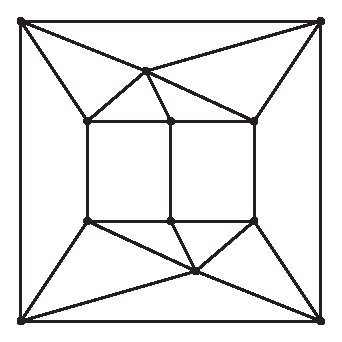
\includegraphics{PS/pentagraph}
\end{center}
%\includegraphics{pentaface}
%\centerline{ \psfig{file=pentaface.eps} }
\caption{The plane graph of a pentahedral prism.}
\label{fig:pentagraph}
\end{figure}

An example of an arrangement with such a graph is depicted in Figure~\ref{fig:penta2}.

\begin{figure}
\begin{center}
\includegraphics{PS/pentaballs}
\end{center}
%\centerline{ \psfig{file=pentaballs.eps} }
\caption{Spheres in a pentahedral prism arrangement.}
\label{fig:penta2}
\end{figure}

A pentahedral prism is characterized by the arrangement and
combinatorics of its standard regions.  It is composed of ten triangular
standard regions, and five quadrilateral standard regions.

The ten triangles are arranged in two
{\em pentahedral caps}, five triangles arranged around a common vertex.
The five quadrilaterals lie in a band between the two caps.
See Figure~\ref{fig:pentaface}.

\begin{figure}
\begin{center}
\includegraphics{PS/pentaface}
\end{center}
%\centerline{ \psfig{file=pentaface.eps} }
\caption{The faces of a pentahedral prism.}
\label{fig:pentaface}
\end{figure}

Recall that the standard cluster attached to a triangular standard region
is a \qrtet.  Likewise, the standard cluster attached to a
quadrilateral is a quad cluster.
We use the term pentahedral cap to refer to
both the standard regions and the \qrtets\ which comprise it.

%\begin{remark}
%In the earliest formulation,  pentahedral prisms
%could score more than $8 \myscorept$.  Pentahedral prisms appeared, on an experimental
%basis, to be the only counterexamples to the potential success of
%the Hales program.  To a certain degree, the pursuit of a proof  that such stars score less than
%$8 \myscorept$ drove the evolution of both the decomposition of space and the
%scoring function.

%Pentahedral prisms still come remarkably
%close to achieving the optimal score of $8 \myscorept$, that achieved by the
%decomposition stars of the face-centered cubic lattice packing.
%In this sense, we consider pentahedral prisms
%to be ``worst case" decomposition stars.

%Thus far,
%the relations required to treat pentahedral prisms have been
%delicate in contrast to the more general bounds which have to date
%sufficed to treat other decomposition stars.

%\end{remark}


\section{The Main Theorem}
\label{sec:dabound} We begin by recalling various definitions from
Paper II, Formulation.  The constant $\myscorept$ is introduced in
Definition~\ref{def:pt}\tomcite.  Similarly, {\em score} is defined
in Theorem~\ref{lemma:negligible'}\tomcite, as well as
Definition~\ref{def:sigma}\tomcite\ and
Remark~\ref{remark:vor}\tomcite. We denote the score of a region $R$
by $\myscore(R)$.

\begin{thm}
\label{thm:dabound}
Each pentahedral prism $P$ satisfies
\[\myscore(P) \le (8 - \epsilon_0) \myscorept\]
for $\epsilon_0 = 10^{-8}$.  Hence there are no contravening pentahedral prisms.
\end{thm}

The next section will introduce a series of propositions which will prove the main theorem.
The first proposition will restrict our attention to a set of potentially contravening pentahedral prisms.
Subsequent propositions  will provide a collection of relations which we will use to prove the main theorem.

\section{Propositions}
\label{sec:props} The function $sol(\cdot)$ is introduced in
Definition~\ref{def:sol}\tomcite.  The function $dih(\cdot)$ is
introduced in Definition~\ref{def:dih}\tomcite.

We present computations using auxiliary bounds
which imply the main result of the paper, that the
score of any pentahedral prism is strictly less than $8 \myscorept$.

Recall from Section~\ref{sec:ssc}\tomcite\ that the score
decomposition for a decomposition star $S$ takes the form
\[\myscore(S) = \sum_R\myscore(R)\]
where $R$ runs over the standard clusters in $S$.

In the case of a pentahedral prism $P$, the score $\myscore(P)$ decomposes
as
\[\myscore(P) = \sum_{i=1}^{10}\myscore(T_i) + \sum_{j=1}^5\myscore(Q_j)\]
with the triangular regions $T_i$ numbered so that the two pentahedral
caps $C_i$ consist of $\{T_i: 1 \le i \le 5\}, \{T_i : 6 \le i \le 10\}$ and $Q_j$ denote
the quad clusters.  Thus
\[ \myscore(C_1) = \sum_{i=1}^5 \myscore(T_i), \text{ \ \ \ } \myscore(C_2) = \sum_{i=6}^{10} \myscore(T_i).\]

% The argument for the nonexistence of a contravening configuration is by contradiction.
% We assume there exists a pentahedral prism with score at least $8 \myscorept$ and derive inequalities % showing that its score is strictly less than $8 \myscorept$.  This proves no such decomposition star exists.

The following proposition gives basic inequalities which we will use to form a restricted set of
pentahedral prisms.

%We use the following lemma to restrict our attention to potentially contravening pentahedral
%prisms.

\begin{prop}
\label{prop:pentscorebd}
A pentahedral prism $P$ satisfies the bound
\[\myscore(P) \le (8 - \epsilon_0) \myscorept\]
for $\epsilon_0 = 10^{-8}$ provided that any one of the following conditions holds:
\begin{enumerate}
\item $P$ contains a tetrahedron $T$ such that
    \[\myscore(T) \le -0.52 \myscorept\] \label{eq:triangle}
\item $P$ contains a quad cluster $Q$ such that
    \[\myscore(Q) \le -1.04 \myscorept\] \label{eq:quad}
\item $P$ contains a pentahedral cap $C$ such that
    \[\myscore(C) \le 3.48 \myscorept\]  \label{eq:penta}
\end{enumerate}
\end{prop}

%\begin{  enumerate}
%item Triangular regions score $ -0.52 \myscorept$
%\item Quad clusters score $> -1.04 \myscorept$
%\item Pentahedral caps score $> 3.48 \myscorept$
%\end{enumerate}
%\begin{eqnarray}
% \myscore(T) & > & -0.52 \myscorept   \label{eq:triangle}   \\
% \myscore(Q) & > & -1.04 \myscorept  \label{eq:quad}        \\
% \myscore(C) & > & 3.48 \myscorept   \label{eq:penta}
%\end{eqnarray}

\begin{proof}
We use the following scoring bounds proved earlier for any admissible decomposition star.

First, Lemma~\ref{lemma:1pt}\tomcite\ states that any \qrtet\ $T$
satisfies
    \[\myscore(T) \le 1 \myscorept. \]

Theorem~\ref{lemma:quad0}\tomcite\ states that any quad cluster $Q$
satisfies
    \[\myscore(Q) \le 0.\]

Next, a pentahedral cap $C$ consists of five quasi-regular
tetrahedra $T_i$ sharing a common distinguished edge.  At one end of
the distinguished edge is the distinguished vertex $v=0$ which is
the center of the decomposition star $P$.  Each $T_i$ has context
$c_i = (5, 0)$. Lemma~\ref{lemma:0.55}\tomcite\ (with $k=1$ and
$r=5$) and Lemma~\ref{lemma:0.55A}\tomcite\ state that any
pentahedral cap $C_i$ satisfies
    \[\myscore(C_i) = \sum_{i=1}^5 \myscore(T_i,c_i,v) \le (4.52 - \epsilon_0) \myscorept\]
with $\epsilon_0 = 10^{-8}$.

\begin{enumerate}
\item Suppose that some $\myscore(T) \le -0.52 \myscorept$, with $T$ contained in a pentahedral cap $C_1$.
Then the inequalities above give
\begin{eqnarray*}
\myscore & \le & -0.52 \myscorept + 4(1 \myscorept) + \myscore(C_2) + \sum_{j=1}^5\myscore(Q_j)    \\
                 & \le & 3.48 \myscorept  + (4.52 - \epsilon_0) \myscorept + 5(0) = (8 - \epsilon_0) \myscorept
\end{eqnarray*}

\item Suppose that some quad cluster $\myscore(Q_j) \le -1.04 \myscorept$.  Then
\begin{eqnarray*}
\myscore(P) & \le & \myscore(C_1) + \myscore(C_2) + (-1.04 \myscorept) + 4(0)    \\
                 & \le & 2((4.52 - \epsilon_0) \myscorept) -(1.04 \myscorept) = (8 - 2\epsilon_0) \myscorept
\end{eqnarray*}
\item Suppose that some pentahedral cap $C_1$ has $\myscore(C_1) \le 3.48 \myscorept$.
Then the inequalities above give
    \[\myscore(P) \le (3.48 \myscorept) + (4.52 - \epsilon_0) \myscorept + 5(0) = (8 - \epsilon_0) \myscorept\]
\end{enumerate}

This completes the proof.
\end{proof}

%\begin{cor}
%\label{cor:pentscorebd}
%The score of any  pentahedral prism excluded by
%Proposition~\ref{prop:pentscorebd} is bounded above by
%$(8 - \epsilon) \myscorept$ for a fixed constant $\epsilon > 0$.
%Therefore, a pentahedral prism excluded by Proposition~\ref{prop:pentscorebd}
%cannot contravene.
%\end{cor}
%
%\begin{proof}
%This is a side-effect of the proof of Proposition~\ref{prop:pentscorebd}.
%\end{proof}
%
%We restrict our attention to pentahedral prisms not excluded
%by  Proposition~\ref{prop:pentscorebd}.

\begin{defn}
\label{defn:pcpp}
% A {\em PC pentahedral prism} is a pentahedral prism which is not excluded by
% Proposition~\ref{prop:pentscorebd}, namely, it is a potentially contravening pentahedral
% prism such that none of (1)-(3) hold.

% (1) [Defn. 15.1] Add at end : "A [strict PC pentahedral prism] is one
%  in which (1), (2), (3) each hold with strict inequality."

A {\em PC pentahedral prism} is a pentahedral
prism such that
\begin{enumerate}
  \item All tetrahedra $T$ have $\myscore(T) \ge -0.52 \myscorept$ \label{defn:pcpp:a}
  \item All quad clusters have $\myscore(Q) \ge 1.04 \myscorept$ \label{defn:pcpp:b}
  \item All pentahedral caps have $\myscore(C) \ge 3.48 \myscorept$ \label{defn:pcpp:c}
\end{enumerate}
and the configuration arises as a pointwise limit
of configurations in which (\ref{defn:pcpp:a}), (\ref{defn:pcpp:b}), (\ref{defn:pcpp:c}) hold with
strict inequality. A  {\em strict PC pentahedral prism} is one in which
(\ref{defn:pcpp:a}), (\ref{defn:pcpp:b}), (\ref{defn:pcpp:c}) each hold with strict inequality.
\end{defn}

All remaining propositions will apply to PC pentahedral prisms.  This restriction improves the
quality of the bounds which we are able to prove on components of a pentahedral prism.

The following two propositions contain linear relations which will imply
the main theorem.
We defer their proofs to the next section.

\begin{prop}
\label{prop:qrtetbound}
For a \qrtet\ $T$ in a PC pentahedral prism, the following
linear inequality holds between $\myscore(T)$, the spherical angle $\sol(T)$
(at the central vertex common to the five tetrahedra in the pentahedral cap),
and the dihedral
angle $\dih(T)$ associated with the first edge of the tetrahedron
(that is, the edge common to the  five tetrahedra in a pentahedral cap):
\[\myscore(T) + m \sol(T) + a (\dih(T) - \frac{2 \pi}{5}) - b_c \le 0\]
Here $a = 0.0739626$, $b_c = 0.253095$, and $m = 0.3621$.
%tetshift[x_]:= 0.253095 - 0.3621*x (eps = 0.0739626)
\end{prop}

\begin{prop}
\label{prop:quadbound}
For a quad cluster $Q$ in a PC pentahedral prism, the following linear inequality holds
between $\myscore(Q)$ and the spherical angle $\sol(Q)$:
\[ \myscore(Q) + m \sol(Q) - b_q \le 0, \]
Here $b_q = 0.49246$ and again $m = 0.3621$.
%line1[x_]:= 0.4922197796533495 - 0.3621*x
\end{prop}

From Propositions \ref{prop:qrtetbound} and \ref{prop:quadbound} we can deduce
the following theorem.
% We now present the main result of this paper.

\begin{thm}
\label{thm:dapcbound}
Each PC pentahedral prism  $P$ satisfies the score bound
    \[ \myscore(P) \le 7.9997 \myscorept \].
\end{thm}

\begin{proof}
Propositions~\ref{prop:qrtetbound} and \ref{prop:quadbound} provide linear relations on all of the
standard clusters in a PC pentahedral prism $P$.
We combine these relations to prove the required score bound.

Invoking Proposition~\ref{prop:qrtetbound} for the five \qrtets\ $\{T_i: i=1\dots 5\}$
from a pentahedral cap, we find
\[
\sum_{i=1}^5 \myscore(T_i) + m \sum_{i=1}^5 \sol(T_i) +
a \sum_{i=1}^5 (\dih(T_i) - \frac{2 \pi}{5}) - 5 b_c \le 0.
\]
Summing over both pentahedral caps and using the relation that
the sum of the five dihedral angles in a pentahedral cap is $2 \pi$,
\[
\sum_{i=1}^5 \dih(T_i) = 2 \pi,
\]
we find
\[
\sum_{i=1}^{10} \myscore(T_i) + m \sum_{i=1}^{10} \sol(T_i) - 10 b_c \le 0.
\]
We represent the tetrahedra from the second
pentahedral cap by the indices $i=6 \ldots 10$.

Invoking Proposition~\ref{prop:quadbound} for
the five quad clusters $\{Q_i: i=11\ldots 15\}$,
and using the fact that the sum of the solid
angles is $4 \pi$,
\[
 \sum_{i=1}^{10} \sol(Q_i) + \sum_{j=11}^{15} \sol(Q_j) = 4 \pi
\]
we find
\[
\sum_{i=1}^{10} \myscore(T_i)  + \sum_{j=11}^{15} \myscore(Q_j) +
4 \pi m - 5 b - 10 b_c \le 0.
\]

Therefore,
\[
\myscore(P) \le 5 b + 10 b_c - 4 \pi m.
\]
% The left-hand side denotes the score of a pentahedral prism.
% If the right-hand side is bounded below $8 \myscorept$, we have achieved the required result.
Substituting the values of $b, b_c, m, \text{ and } \myscorept$, we find that the
score of a PC pentahedral prism is less than $7.9997 \myscorept$.
\end{proof}

% In the cases covered by Proposition~\ref{prop:pentscorebd},
% we have the scoring bound $(8 - \epsilon) \myscorept$, from Corollary~\ref{cor:pentscorebd}.
%
% In either case, this contradicts our assumption that contravening pentahedral prisms exist,
% therefore there are no contravening pentahedral prisms.

Assuming Proposition~\ref{prop:pentscorebd} and Theorem~\ref{thm:dapcbound} we can prove
Theorem \ref{thm:dabound}.

\begin{proof}
Given a pentahedral prism $P$, it is either PC or it is not.  In the former case,
its score is bounded by $7.9997 \myscorept$.  In the latter case, its score is bounded
by $(8 - 10^{-8}) \myscorept$.  In both cases, its score is bounded by $(8 - 10^{-8}) \myscorept$.
\end{proof}

\begin{remark}
The score  bound in Theorem~\ref{thm:dabound} is weaker than what is possible to prove.  In the interest of simplifying the exposition as well as the required computations, we establish this weaker bound which suffices for this part of the proof of the Kepler conjecture.

% A proof of Theorem~\ref{thm:dabound}
% with a better bound would require careful treatment of a number of special cases which do not arise in % our current approach.  The inequalities which would arise in such an approach would differ from
% those which suffice in our case.
\end{remark}

\chapter{The Main Propositions}

In the first section, we recall the definition of score, and introduce some local notation.  In the next section, we recall the notion of dimension reduction, and prove its validity for some relevant cases.
In the following section, we prove Proposition~\ref{prop:qrtetbound}.
In the remaining sections we prove Proposition~\ref{prop:quadbound}.
% We prove Proposition~\ref{prop:quadbound} independently for all possible kinds of quad clusters
% (and their associated scoring schemes):
% \begin{enumerate}
% \item Flat quad clusters
% \item Octahedra
% \item Truncated Voronoi clusters
% \item Mixed quad clusters
% \end{enumerate}
% Each of these cases will be treated in its own section, except for truncated Voronoi clusters, which
% have additional sections treating the acute and obtuse cases.

\section{Scoring}
The development of a scoring function is central to the proof of the Kepler conjecture.  Its
definition is therefore somewhat complicated.  Fortunately, in our treatment of the
pentahedral prism we are able to restrict our attention to only a few cases in
the scoring system.

Recall that {\em score} is defined in
Theorem~\ref{lemma:negligible'}\tomcite, as well as
Definitions~\ref{def:svor} and \ref{def:sigma}\tomcite\ and
Remark~\ref{remark:vor}\tomcite{}. See
Remark~\ref{remark:score}\tomcite\ for a simplified version of the
scoring function for quarters.

In our context, the score $\myscore(\cdot)$ breaks into four different scoring types:
$gma(\cdot)$, $vor(\cdot)$, $octavor(\cdot)$, and Voronoi.

$gma(\cdot)$ applies to \qrtets\ and quarters, and is introduced as
$\Gamma(\cdot)$ in Definition~\ref{def:svor}\tomcite{}.  We
frequently use the term {\it compression\/} as an alias for
$\gma(\cdot)$.  This alias was introduced in \Chap~\ref{def:svor}.

$vor(\cdot)$ is the score determined by the analytic continuation of
the Voronoi volume associated with the distinguished vertex of a
tetrahedron, and corresponds to $s\text{-}vor(\cdot)$ in
Definition~\ref{def:svor}\tomcite{}.

We let $octavor(\cdot)$ denote the score of an upright quarter in context (4,0) which is
not scored by compression.  In this case, $octavor(\cdot)$ is the average of two $vor(\cdot)$ scores.

Voronoi scoring, which we also refer to as pure Voronoi scoring, is
$vor_R(D)$ from Remark~\ref{remark:vor}\tomcite{}.


\section{Dimension Reduction}
The relations on tetrahedra required for
the scoring bound on decomposition stars are typically
six-dimensional, as they are formulated in terms of
the edge lengths of a tetrahedron.  For a quad cluster, they can be even
higher-dimensional.  For high-dimensional relations,
the method of subdivision becomes very expensive,
computationally speaking.

We define a simplification which reduces the dimension
of the required computations.  This simplification
therefore reduces the computational expense of the
verification of a relation.

We refer to this simplification as dimension-reduction.  We will
apply this simplification for three different scoring types:
compression, vor analytic, and Voronoi. These scoring functions are
introduced in Definitions~\ref{def:svor}\tomcite\ and
\ref{def:sigma}\tomcite. See Remark~\ref{remark:score}\tomcite\ for
a simplified version of the scoring function for quarters.

\begin{thm}
\label{thm:dimred}
(Dimension-reduction)  Given a tetrahedron $T$ with a fixed scoring type
(one of compression, vor analytic, or Voronoi),
the deformation
consisting of moving a vertex $v_i$ along the edge $(0, v_i)$ towards the origin increases the
score of the tetrahedron.
\end{thm}

Note that this deformation holds the solid angle at the origin fixed.  See Figure~\ref{fig:tet}.
Since the reduction may be performed until either a scoring system or an edge-length constraint
is met, this argument reduces the number of free
parameters for the verification, thus reducing the dimension and
complexity of the verification of a relation.

\begin{figure}
\begin{center}
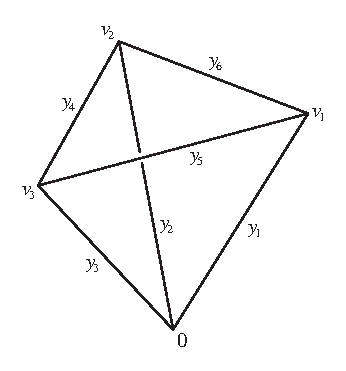
\includegraphics{PS/tet}
\end{center}
\caption{Tetrahedron with distinguished vertex and labeled edges.}
\label{fig:tet}
\end{figure}

\begin{proof}
There are three cases to consider: compression scoring, vor analytic
scoring and Voronoi scoring. This technique was introduced in
Proposition~8.7.1 of \cite{part1} for compression-scoring, and is
proved there in the compression case.

Next we consider vor analytic-scored tetrahedra.  The validity of
the same reduction for vor analytic-scored tetrahedra is obvious if
the tip of the Voronoi cell does not protrude. If the tip does
protrude, we must use the analytic continuation for the Voronoi
volume.  In this case, the validity of the reduction is not obvious.

% We provide an analytic proof (with some details omitted) that this reduction increases
% the analytic Voronoi score of a tetrahedron.
The geometric constraint of moving a vertex along an edge
can easily be stated analytically in terms of the original edge
lengths, $(y_1, y_2, y_3, y_4, y_5, y_6)$.
This action depends on a single parameter, the
distance of the vertex $v_1$ from the origin, which we call $t$.
The new edge lengths are given by
\[
( t, y_2, y_3,
  y_4,\sqrt{{t^2} + {{{y_3}}^2} -
   {\frac{t\,\left( {{{y_1}}^2} +
         {{{y_3}}^2} - {{{y_5}}^2}
         \right) }{{y_1}}}},
  \sqrt{{t^2} + {{{y_2}}^2} -
   {\frac{t\,\left( {{{y_1}}^2} +
         {{{y_2}}^2} - {{{y_6}}^2}
         \right) }{{y_1}}}} ).
\]

Recall from Section~8.6.3 of \cite{part1} that the formula for the
analytic Voronoi volume is a rational function of $\chi$, $u$,
$\sqrt{\Delta}$, and $x_i$, where $x_i = y_i^2$.  Further recall
that $\chi$, $u$, and $\Delta$ are all polynomial functions in $x_i$
that are defined in Sections~8.1 and 8.2 of \cite{part1}.

Substituting the computed edge lengths in the formula for the analytic
Voronoi volume, taking the partial derivative with
respect to $t$, replacing $t$ with $y_1$, multiplying by the positive
term
\[
8 \sqrt{\Delta} u(x_1, x_3, x_5) u(x_1, x_2, x_6)/y_1,
\]
and then simplifying, we end up with a large homogeneous
polynomial in $x_i$ of degree 6, which is too ugly to exhibit here (having
91 terms).

Evaluating this polynomial over all possible
\qrtets\ and quarters, we find that it is positive.

Therefore the volume is increasing in $t$, so to increase the score,
we should push the vertex in along the edge. The verification of the
sign of the polynomial is found in Calculation~\ref{d:dimred}. This
completes the case of vor analytic-scored tetrahedra.

The final case is Voronoi scoring.  The deformation does not change
the solid angle of the tetrahedron.  The only term of the Voronoi
score that changes is a negative constant times a volume. The
contraction of the tetrahedron decreases this volume, and increases
the score. The validity of a similar reduction argument for Voronoi
scoring of a tetrahedron is now obvious.
\end{proof}


\section{Proof of Proposition~\ref{prop:qrtetbound}}
%\section{Quasi-regular Tetrahedra}
%Otherwise known as the pentahedral cap.
% \subsection{Quasi-regular Tetrahedra}

%     Add at beginning a new paragraph: "It suffices to prove
%  Proposition 15.2 for strict PC pentahedral prisms. For each
%  non-strict PC pentahedral prism is a pointwise limit of strict
%  ones of the same combinatorial type, so the inequality in
%  the conclusion of the proposition will hold for non-strict
%  PC pentahedral prisms by continuity."

    It suffices to prove
 Proposition~\ref{prop:qrtetbound} for strict PC pentahedral prisms. Each
 non-strict PC pentahedral prism is a pointwise limit of strict
 ones of the same combinatorial type, so the inequality in
 the conclusion of the proposition will hold for non-strict
 PC pentahedral prisms by continuity.

We use three separate computations to construct and prove Proposition~\ref{prop:qrtetbound}.
First, we prove a relation between dihedral
angle and score.  We then show that if the dihedral angle of a
tetrahedron in a pentahedral cap exceeds a certain bound,
then the associated pentahedral prism is not a strict PC pentahedral prism.
% the score of the pentahedral cap must fall below $3.48 \myscorept$,
% hence such arrangements may be discarded.
% falling into the purview of Proposition~\ref{prop:pentscorebd}.
We call such a bound a
{\em dihedral cutoff}.  This cutoff allows us to prove the final bound.

%  Replace "cannot contravene." with "is not a strict PC pentahedral prism."

In the following discussion, $\dih(T)$ refers to the dihedral angle
associated with the first edge of a \qrtet\ $T$, $\myscore(T)$ refers to
the compression score of the tetrahedron,
and $\sol(T)$ refers to the solid
angle at the distinguished vertex.  We restrict
our attention to \qrtets\ whose score exceeds $-0.52 \myscorept$, as
otherwise the associated pentahedral prism cannot contravene.
% per Proposition~\ref{prop:pentscorebd}.

The first relation is
%$$\myscore(T) \le a_1 \dih(T) - a_2$$
\begin{eqnarray}
\myscore(T) \le a_1 \dih(T) - a_2  \label{eq:qr:dihrel}
\end{eqnarray}

where $a_1 = 0.3860658808124052$ and $a_2 = 0.4198577862$.
Calculation~\ref{qr:dihrel}
provides the verification of this relation.

%smside2[tt_]:= -0.4198577860315257 + 0.3860658808124052*tt

% If a pentahedral prism has a  pentahedral cap that contains
%  a quasi-regular tetrahedron with dihedral angle dih(T) \ge d_0,
%  where d_0=1.4674, then it is not a strict PC pentahedral prism."

\begin{lem}
\label{lem:dihcut}
If a pentahedral prism has a pentahedral cap that contains a \qrtet\ $T$ with
dihedral angle $\dih(T) \ge d_0$,
where $d_0 = 1.4674$, then it is not a strict PC pentahedral prism.
% we can discard it via Proposition~\ref{prop:pentscorebd}.
\end{lem}

\begin{proof}
Applying relation (\ref{eq:qr:dihrel}) to four \qrtets\ $T_i$ forming part of a strict PC pentahedral
prism, we find
\begin{eqnarray}
\sum_{i=1}^4 \myscore(T_i) \le a_1 \sum_{i=1}^4 \dih(T_i) - 4 a_2 \label{eq:qr:dihsum}
\end{eqnarray}
Applying the relation
\begin{eqnarray}
\dih(T_5) = 2 \pi - \sum_{i=1}^4 \dih(T_i) \label{eq:qr:dihsum2}
\end{eqnarray}
and adding $\myscore(T_5)$ to both sides of relation (\ref{eq:qr:dihsum}),
we find
\begin{eqnarray}
\sum_{i=1}^5 \myscore(T_i) \le \myscore(T_5) + a_1 (2 \pi - \dih(T_5)) - 4 a_2 \label{eq:qr:dihsum3}
\end{eqnarray}
The left-hand side represents the score of the pentahedral cap.
If the right-hand side does not exceed $3.48 \myscorept$,
then the pentahedral prism is not a strict PC pentahedral prism.
% Proposition~\ref{prop:pentscorebd} implies that the associated
% pentahedral prism cannot contravene.
 % (line 9) replace "Proposition 15.1 implies... cannot contravene."
 % with: " then the pentahedral prism is not a strict PC pentahedral prism.

% we can remove the arrangement from consideration,  as per Proposition~\ref{prop:pentscorebd}.

%d_0 = 1.4674

We assert that if $\dih(T) \ge d_0$,
the right-hand side
\[
\myscore(T_5)  + a_1 (2 \pi - \dih(T_5)) - 4 a_2
\]
does not exceed $3.48 \myscorept$.  Equivalently,
we prove that
$\dih(T) \ge d_0$ implies
\[
\myscore(T) - a_1 \dih(T) \le 3.48 \myscorept - 2 \pi a_1 + 4 a_2
\]
which is verified in Calculation~\ref{qr:dihcut}.

We conclude that if $\dih(T) \ge d_0$
 then the pentahedral prism cannot be a strict PC pentahedral prism.

\end{proof}

Hence we may restrict our attention to \qrtets\ whose
dihedral angle does not exceed the dihedral cutoff $d_0$.

Using the dihedral cutoff, we establish the final relation,
\[\myscore(T) + m \sol(T) + a (\dih(T) - \frac{2 \pi}{5}) - b_c \le 0\]
via Calculation~\ref{qr:pentacap}.  This completes the proof of Proposition~\ref{prop:qrtetbound}.

\section{Proof of Proposition~\ref{prop:quadbound}: Top level}

 It suffices to prove
 Proposition\ref{prop:quadbound} for strict PC pentahedral prisms,
 by a similar argument to that used for Proposition~\ref{prop:qrtetbound}.

Recall from Definition~\ref{def:standard-cluster}\tomcite{}
%of \cite{dcg2}
that a quad cluster is
a standard region that is a quadrilateral.
Quad clusters can be classified as follows:

\begin{enumerate}
 \item Flat quad clusters \label{enum:class:flat}
 \item Octahedra \label{enum:class:octa}
 \item Pure Voronoi quad clusters \label{enum:class:vor}
 \item Mixed quad clusters \label{enum:class:mixed}
\end{enumerate}

We will subdivide (\ref{enum:class:vor}) into acute and obtuse types.
See Section~\ref{sec:bounds}\tomcite{} %of \cite{dcg3} 10.4
for a discussion on the classification of quad clusters.
% make sure these references match up, as per Jeff's comments
By Lemma~\ref{lemma:1.04}\tomcite{}, the score of a mixed quad
cluster is less than $-1.04 \myscorept$. A PC pentahedral prism
therefore cannot contain a mixed quad cluster, so the bound of
Proposition~\ref{prop:quadbound} holds trivially for this class.

We treat the remaining classes in the following sections.

\section{Proof of Proposition~\ref{prop:quadbound}: Flat quad clusters}

Recall that a {\em flat} quarter is a quarter whose long edge is opposite its distinguished vertex.

\begin{lem}
\label{lem:flatquarterbd}
Given a flat quarter $Q$ with $\myscore(Q) \ge -1.04 \myscorept$, the relation
\begin{eqnarray}
\myscore(Q) \le -m \sol(Q) + b/2  \label{rel:flatquarterbd}
\end{eqnarray}
holds.
\end{lem}

\begin{proof}
Label the diagonal of a flat
quarter $y_6$.

Flat quarters may be scored using either compression or vor
scoring.  We treat each case separately.

First, suppose that we wish to prove the bound for compression scored
quarters.  This means that the circumradii of the two faces adjacent
to the long diagonal do not exceed $\sqrt{2}$.  We subdivide the
verification into
Calculation~\ref{flat:gma:dimred},
a computation where we apply dimension-reduction
and partial derivative information, and
Calculation~\ref{flat:gma:bdry}, a boundary verification, where
we restrict our attention to cells which lie on the boundary between
compression and vor scoring.

%Calculation~\ref{flat:gma:dimred} provides the verification
%of the dimension-reduction
%case.  Calculation~\ref{flat:gma:bdry} provides the
%verification of the boundary case.

Second, we treat the vor-scoring case.  In this case we prove the
bound for vor-scored quarters.  This means that at least one of
the circumradii of the two faces adjacent to the long diagonal
is at least $\sqrt{2}$.  This verification is somewhat more complex
than the compression case.  We subdivide the verification into
\begin{enumerate}
\item
Verification that the first three partials are negative on a
small cell containing the corner (Calculation~\ref{flat:partials}).
\item
Verification of the bound on that small cell containing the corner,
using the property that the first three partials are negative
(Calculation~\ref{flat:corner}).
\item
A computation where we apply dimension-reduction and partial
derivative reduction, omitting the corner cell
(Calculation~\ref{flat:vor:dimred}).
\item
A boundary verification, where we restrict our attention to
cells which lie on the boundary between compression and vor
scoring, again omitting the corner cell
(Calculation~\ref{flat:vor:bdry}).
\end{enumerate}

These calculations complete the proof of Lemma~\ref{lem:flatquarterbd}.
\end{proof}

We are now prepared to prove Proposition~\ref{prop:quadbound} for flat quad clusters.

Flat quad clusters are composed of two flat quarters, whose common face
includes the long edge.

By Proposition~\ref{prop:pentscorebd}, we restrict our attention to
flat quarters whose score exceeds $-1.04 \myscorept$, recalling the
fact that the score of flat quarters is nonpositive.

Invoking Lemma~\ref{lem:flatquarterbd} for each flat quarter and adding the relations,
we arrive at the desired
bound for flat quad clusters.  This completes the proof.

%These verifications are contained in Calculations (ref.).

\section{Proof of Proposition~\ref{prop:quadbound}: Octahedra}

% \subsection{Octahedra}
%Four upright quarters, arrayed around their common long edge so
%that each face containing the common edge is shared by two quarters,
%form an {\em octahedron}, another type of quad cluster.

Recall that quartered octahedra, a type of quad cluster,
are composed of four upright
quarters arrayed around their common long edge
(called the {\em diagonal}) so that each
face containing the common edge is shared by two quarters.

We are required to prove a relation of the form
\[ \myscore(H) + m \sol(H) - b \le 0, \]
where $\myscore(H)$ denotes the score of an octahedron $H$, $\sol(H)$ denotes
the solid angle associated with the distinguished vertex, and $m$
and $b$ are positive constants.  By Proposition~\ref{prop:pentscorebd},
we restrict our attention to
octahedra whose score exceeds $-1.04 \myscorept$.

Our treatment of octahedra, as usual, is comprised of a number of auxiliary
computations.  We prove bounds on upright quarters which are part of an
octahedron, and then combine these bounds to deduce the required bound on
octahedra in general.

The scoring function $\myscore(\cdot)$ for upright quarters is either compression
(denoted by $\gma(\cdot)$) or
an average of two $\vor(\cdot)$ scores, which we will continue to refer to as
vor-scoring.
See Remark 7.23 for a simplified version of the scoring rules.

Due to the complex nature of octahedra, we
consider a number of sub-cases.
These cases are partitioned according to the length
of the diagonal and the scoring system applied to the upright quarters.

Using a dihedral summation argument, we will eliminate octahedra
whose diagonal lies in the range $[2.51, 2.716]$.

Next, we will treat
the case where the diagonal lies in the range $[2.716, 2\sqrt{2}]$.
Using a dihedral correction term,
we will prove the bound for octahedra which are completely
compression-scored, and octahedra which are completely vor-scored.

The remaining cases will consist of
octahedra which contain either two or three
vor-scored quarters.  (Since a quarter is vor-scored if one
of the faces containing the diagonal has circumradius $\sqrt{2}$ or
greater, it is not possible for an octahedron to contain only one
vor-scored quarter.)  We treat these cases using an additional
correction term.

In all computations involving octahedra,
we label the diagonal $y_1$.

In order to simplify the computations,
we first prove an auxiliary cutoff bound.
This first bound reduces
the size of the cell over which we must conduct our search,
as per Proposition~\ref{prop:pentscorebd}.

\begin{lem}
\label{lem:octa:peel} If an upright quarter contains an edge
numbered 2, 3, 5, or 6 whose length is not less than $2.2$, its
score is less than or equal to $-0.52 \myscorept$.
\end{lem}

\begin{proof}
This is Calculation~\ref{octa:peel}.
\end{proof}

Since such an edge is shared by another upright quarter
in the same octahedron, the score of the
associated octahedron must fall below $-1.04 \myscorept$.

We restrict our search accordingly.

%Octahedral cutoff:  show that if the diagonal of an
%octahedron lies in the range [2.51,2.71], the score of
%the octahedron is less than -1.04 pt.  Hence, we can
%discard such arrangements.
%Specifically, we verify the following bound to within
%a tolerance of (fill_in_the_blank):
%sc < m*dih + b,
%where
%Newer version:  cutoff = 2.716,
%{m, b} = {-0.1533667634670977, 0.2264803995076098}
%Required tolerance (for the new bound):  3.0e-5

\begin{lem}
\label{lem:octa:2716}
The score of an octahedron $H$ with upright diagonal in the range $[2.51, 2.716]$
is less than or equal to $-1.04 \myscorept$.
\end{lem}

\begin{proof}
In Calculation~\ref{octa:cut},
we prove a bound of the form
\[
\myscore(S) + c \dih(S) \le d
\]
on upright quarters $S$, where $c = 0.1533667634670977$, and
$d = 0.2265$.  Adding the bound for four quarters $S_i$ forming
an octahedron, we find
\[
\sum_{i=1}^4 \myscore(S_i) + c \sum_{i=1}^4 \dih(S_i) \le 4 d.
\]
Using the fact that the sum of the dihedral angles is $2 \pi$,
we find that
\[
\myscore(H) \le -2 \pi c + 4 d
\]
for such an octahedron $H$.

A computation involving the constants $c$ and $d$ shows that the
score is less than $-1.04 \myscorept$.
\end{proof}

Again invoking
Proposition~\ref{prop:pentscorebd}, we need only
consider octahedra whose diagonal lies in the range
$[2.716, 2\sqrt{2}]$.

%Next, we consider octahedra which contain (at least two)
%vor-scored quarters whose diagonal falls in the range
%$[2.716, 2.81]$.  We prove a cutoff bound, showing that
%a vor-scored quarter with such a diagonal must score
%less than $-0.52 \myscorept$.  Since there must be at least
%two such quarters if there are any, the score of the
%octahedron with which they are associated must fall below
%$-1.04 \myscorept$.  We therefore discard such arrangements,
%restricting our attention to diagonals in the range

Using this assumption, we prove bounds of the form
\begin{equation}
%\[
\myscore(S) + m \sol(S) + \alpha \dih(S)  \le \frac{b}{4} +
    \alpha \frac{\pi}{2}
%\]
\label{octa:dih}
\end{equation}
and
\begin{equation}
%\[
\myscore(S) + m \sol(S) + \alpha \dih(S) + \beta x_1 \le \frac{b}{4} +
    \alpha \frac{\pi}{2} + 8 \beta,
%\]
\label{octa:edge}
\end{equation}
where $\dih(S)$ refers to the dihedral angle associated with the diagonal,
$\myscore(S)$ refers to the scoring scheme appropriate for a
particular upright quarter $S$, and $x_1$ refers to the square of the length of
the diagonal.  We
choose $\alpha$ and $\beta$ according to the scoring scheme.

Appropriate values for the correction terms involving
$\alpha$ and $\beta$ were determined by experimentation.

%For the first inequality, we choose $\alpha = 0.14$ for compression-scored
%quarters, and $\alpha = 0.054$ for vor-scored quarters.

%We prove Relation~\ref{octa:dih} for compression-scored quarters, choosing
%$\alpha = 0.14$.

Choosing $\alpha = 0.14$, we prove (\ref{octa:dih}) for compression-scored
quarters with diagonal in the interval $[2.716, 2\sqrt{2}]$
(Calculation~\ref{octa:gma:dih}).  Using
the same $\alpha$, we prove (\ref{octa:dih}) for vor-scored
quarters with diagonal in the range $[2.716, 2.81]$ (Calculation~\ref{octa:vor:dih}).

Choosing $\alpha = 0.054$, $\beta = 0.00455$, we prove (\ref{octa:edge}) for
compression-scored quarters with diagonal in $[2.81, 2\sqrt{2}]$
(Calculation~\ref{octa:gma:corr}).  Choosing
the same $\alpha$, but $\beta = -0.00455$, we prove (\ref{octa:edge}) for
vor-scored quarters with diagonal in $[2.81, 2\sqrt{2}]$
(Calculation~\ref{octa:vor:corr}).

%For the second inequality, we choose $\alpha = 0.054$, and we choose
%$\beta = 0.00455$ for compression-scored quarters, and $\beta = -0.00455$
%for vor-scored quarters.

Note that for vor-scored quarters,
the first inequality is a relaxation of the second, since $\beta$ is
negative.

The verification of each of these inequalities involves
a computation where we apply dimension-reduction
and partial derivative information, and
a boundary verification, where
we restrict our attention to cells which lie on the boundary between
compression and vor analytic scoring.
Note that the
dimension-reduction step for relation~(\ref{octa:edge}) is complicated
by the presence of the $\beta x_1$ term.


\begin{lem}
\label{lem:octabound}
Proposition~\ref{prop:quadbound} holds for octahedra with upright diagonals
in the range $[2.716, 2\sqrt{2}]$.
\end{lem}
\begin{proof}
Summing inequality (\ref{octa:dih}) over the four quarters $S_i$ of an octahedron, we find
\[
\sum_{i=1}^4 \myscore(S_i) + m \sum_{i=1}^4 \sol(S_i) + \alpha \sum_{i=1}^4 \dih(S_i)
\le b + 2 \alpha \pi.
\]
Using the fact that the dihedral angles sum to $2 \pi$, we find
\[
\myscore(H)  + m \sol(H) \le b,
\]
so octahedra $H$ with diagonals in the range $[2.716,2.81]$
satisfy the requisite bound.

Summing inequality (\ref{octa:dih}) over a consistently scored octahedron
(either all compression or all vor) with diagonal in the
range $[2.81, 2\sqrt{2}]$, we again arrive at the desired bound.

The remaining cases involve octahedra which contain both compression
and vor-scored quarters, and whose diagonals lie in the range
$[2.81, 2\sqrt{2}]$.  For this case, we use inequality (\ref{octa:edge}).

The summation involving inequality (\ref{octa:edge}) is identical to
inequality (\ref{octa:dih}) save for
the presence of the $\beta$ terms.  If there are two vor-scored
quarters and two compression-scored quarters, the beta terms cancel,
giving the relation as before.

If there are three vor-scored quarters and one compression-scored
quarter, we note that the same relation for vor-scored quarters
holds if we replace $\beta$ by $\beta/3$ (since we have now relaxed
the bound).  Summing the inequalities, the term involving $\beta$
vanishes again, leaving the desired inequality.
\end{proof}

Lemmas \ref{lem:octa:2716} and \ref{lem:octabound} prove
Proposition~\ref{prop:quadbound} for octahedra.

\section{Proof of Proposition~\ref{prop:quadbound}: Pure Voronoi quad clusters}
% \section{Pure Voronoi quad clusters}

% \subsection{Pure Voronoi quad clusters}
The next class of quad clusters which we treat are the pure
Voronoi quad clusters.  We will define a truncation operation
on these quad clusters.  Truncation will simplify the geometry of
the quad clusters, and will provide a convenient scoring bound.
We will divide our treatment of pure Voronoi quad clusters
into two cases in order to simplify the analysis and numerical
verifications as much as possible.

Recall from the classification of quad clusters
that a pure Voronoi quad cluster consists of the intersection of a
$V$-cell at the origin with the cone at the origin over a quadrilateral
standard region.  We refer to the restriction of the $V$-cell to the
cone over the quadrilateral as either the $V$-cell
or the Voronoi cell of the quad cluster.
Figure~\ref{fig:vor} describes the geometry of a simple
$V$-cell.

\begin{figure}
\begin{center}
\includegraphics{PS/vor}
\end{center}
%\centerline{ \psfig{file=vor.eps} }
\caption{A pure Voronoi quad cluster.}
\label{fig:vor}
\end{figure}

In addition, recall that a vertex lying in the cone over a pure
Voronoi quad cluster must have height greater than $2\sqrt{2}$.
Such vertices can significantly complicate the geometry of the $V$-cell,
affecting its shape and volume.

We remove the effect of vertices lying above a pure Voronoi quad cluster
by removing all points from the $V$-cell which have height greater than
$\sqrt{2}$.  We call this operation {\em truncation at} $\sqrt{2}$.
Truncation decreases the volume of the quad cluster.  This decrease in
volume increases the score of the quad cluster, bringing it closer to
the proposed bound.

We refer to truncated pure Voronoi quad clusters as {\em truncated} quad
clusters.

We define a scoring operation on pure Voronoi quad clusters which we
call {\em truncated Voronoi} scoring.  This operation consists of
truncation at $\sqrt{2}$, followed by the usual Voronoi scoring.

Each diagonal across the face of a cluster must have length
greater than $2\sqrt{2}$, otherwise we could form two flat quarters,
contradicting the decomposition.  We choose the shorter of the two
possible diagonals, and will consider that diagonal in the analysis
which follows.

We decompose the cluster into two tetrahedrons along the chosen
diagonal.  The face dividing the tetrahedrons is either acute or
it is obtuse.  We treat each case separately.

We must prove
\[
\myscore(Q) + m \sol(Q) - b \le 0,
\]
where $\myscore(Q)$ denotes the score of a pure Voronoi quad cluster $Q$, $\sol(Q)$ denotes
the solid angle associated with the distinguished vertex, and $m$
and $b$ are positive constants.
We call this relation a {\em bound} on the solid angle and score of a quad
cluster.
Invoking Proposition~\ref{prop:pentscorebd},
we restrict our attention to
quad clusters whose score exceeds $-1.04 \myscorept$.

% \subsubsection{The acute case}
% \subsection{The acute case}
% \section{Proof of Proposition~\ref{prop:quadbound}: Pure Voronoi quad clusters (acute)}
\section{Pure Voronoi quad clusters:  acute case}
\begin{lem}
\label{lem:pure:half} If an acute quad cluster is divided along an
acute separating face, then the score of each half is nonpositive.
\end{lem}
\begin{proof}
This is a consequence of the arguments of
Theorem~\ref{lemma:quad0}\tomcite.
\end{proof}

We therefore restrict our attention to halves whose score exceeds
$-1.04 \myscorept$, by Proposition~\ref{prop:pentscorebd}.

If the separating face is acute, we prove
\begin{equation}
\myscore(S_i) + m \sol(S_i) - b/2 \le 0 \label{rel:acute}
\end{equation}
for each half $S_i$
independently, and deduce the desired bound by adding the bounds
for each half.

\begin{lem}
\label{lem:pure:solid}
Let $T_0$ denote the tetrahedron with edge lengths $(2,2,2,2,2,2\sqrt{2})$.  Let
$\sol(T_0)$ denote the solid angle of the tetrahedron $T_0$.
Given a tetrahedron $T$, if $\sol(T) < \sol(T_0)$, then relation~(\ref{rel:acute}) holds.
\end{lem}
\begin{proof}
If $\sol(T) < \sol(T_0)$, then
$m \sol(T) < m \sol(T_0)$, hence
\[m \sol(T) -b/2 < m \sol(T_0) - b/2 \le 0,\]
and
\[\myscore(T) + m \sol(T) -b/2 < \myscore(T) \le 0,\]
by Lemma~\ref{lem:pure:half}.
\end{proof}

We therefore
may restrict our attention to halves whose solid angle is at least
$\sol(T_0)$.  In addition, we restrict our attention to halves for
which the dividing face is acute.

\begin{lem}
\label{lem:pure:acute}
The relation \[\myscore(T) + m \sol(T) - b/2 \le 0\] holds for a
tetrahedron $T$ forming  half of an acute quad cluster with
score exceeding $-1.04 \myscorept$.
\end{lem}
\begin{proof}
The required verifications for each half of an acute quad cluster
are somewhat difficult to achieve
directly, so we subdivide into a number of different cases
in an attempt to reduce the complexity of
the calculations.  First, we show that the bound holds for
all halves whose diagonal is at least $2.84$
(Calculation~\ref{acute:cut}).
Using this information, we then prove the
bound everywhere but in a small corner cell
(Calculation~\ref{acute:vor}).  We then restrict our
attention to the small corner cell (Calculation~\ref{acute:corner}).
These computations involve
the use of partial derivative information, and include the required
boundary computations.
\end{proof}

Invoking Lemma~\ref{lem:pure:acute} for each half and adding them proves
Proposition~\ref{prop:quadbound} for the acute case.

\section{Pure Voronoi quad clusters:  obtuse case}
% \section{Proof of Proposition~\ref{prop:quadbound}: Pure Voronoi quad clusters (obtuse)}
% \subsection{The obtuse case}
% \subsubsection{The obtuse case}
If the separating face is obtuse, the analysis becomes significantly
harder.  It is no longer possible to prove the desired bound on each
half independently.  The dimension of the full bound, even using
the usual dimension-reduction techniques, is too high to make the
verification tractable numerically.  Therefore we adopt a different
approach.

Using the dimension-reduction technique, we push each vertex along its
edge until the distance from each vertex to the origin is $2$.
We call the resulting quad cluster a {\em squashed} cluster.  Observe
that the solid angle of the cluster is unchanged, while the volume of
the Voronoi cell has decreased, thereby increasing the score of the
cluster.

Since
the central face is still obtuse, the length of the diagonal after
this perturbation must still exceed $2\sqrt{2}$.  Note, however,
that the other edge lengths in the quad cluster can be as small as
$4/2.51$.

The geometry of the $V$-cell of a squashed cluster, assuming that
there is no truncation from vertices of the packing lying above the quad
cluster, is that of Figure~\ref{fig:vor}.  When the $V$-cell is
truncated at $\sqrt{2}$ from the origin, two potential arrangements
arise.  In the first arrangement, the truncated region is connected,
as in Figure~\ref{fig:vor3}.  In second potential arrangement, the
truncated region is formed of two disjoint pieces,
as in Figure~\ref{fig:vor2}.

\begin{figure}
\begin{center}
\includegraphics{PS/vor3}
\end{center}
%\centerline{ \psfig{file=vor3.eps} }
\caption{A typical truncated quad cluster.}
\label{fig:vor3}
\end{figure}

\begin{figure}
\begin{center}
\includegraphics{PS/vor2}
\end{center}
%\centerline{ \psfig{file=vor2.eps} }
\caption{An impossible arrangement.}
\label{fig:vor2}
\end{figure}

\begin{lem}
\label{lem:pure:disjoint}
The disjoint case cannot arise for squashed quad clusters.
\end{lem}
\begin{proof}
Suppose that it could.  Pick an untruncated point
along the central ridge of the $V$-cell (see Figure~\ref{fig:vor2}).
The distance of this point
from the origin is then less than $\sqrt{2}$, but due to its location
on the central ridge, it is equidistant from the two nearest vertices
and the origin.  This implies that the circumradius of the resulting
triangle must be less than $\sqrt{2}$, which contradicts the fact
that the diagonals have length at least $2\sqrt{2}$.
\end{proof}


\subsection{A geometric argument}
% \subsubsection{A geometric argument}
We introduce a simplification which will reduce the complexity of
the obtuse case.  This simplification will consist of a perturbation of
the upper edge lengths of a squashed quad cluster.  This perturbation
will increase the score while holding the
solid angle of the quad cluster fixed.

This simplification is based on a geometric decomposition of the
truncated Voronoi cell.  We will describe the decomposition, and
then describe a construction which will ultimately simplify the
analysis.

While our arguments will extend to treat a general
squashed and truncated Voronoi cell associated with a general
standard cluster, we restrict our attention to truncated
Voronoi cells associated with quad clusters.

To begin, we consider the decomposition of
a truncated Voronoi cell into its fundamental components.
A truncated Voronoi cell is formed of three elements:  a
central spherical section (formed by the truncation), {\em wedges} of
a right circular cone, and tetrahedrons called {\em Rogers simplices}.

We choose a representation of a truncated quad cluster composed of
the radial projection of each element to a plane passing close to
the four corners of the quad cluster.
This decomposition
is represented in Figure~\ref{fig:quad2}.

\begin{figure}
%\includegraphics{PS/quad2.eps}
\begin{center}
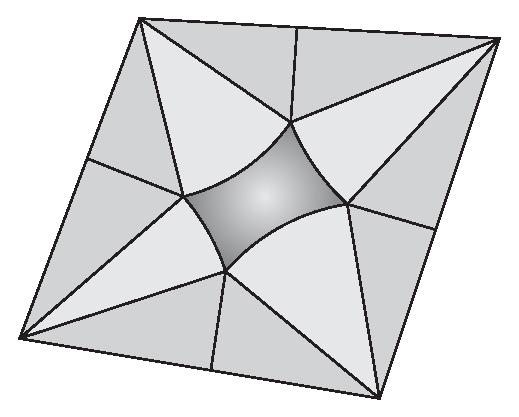
\includegraphics{PS/planar2}
\end{center}
%\centerline{ \psfig{file=quad2.eps} }
\caption{A representation of a truncated quad cluster.}
\label{fig:quad2}
\end{figure}

% \subsubsection{Rogers simplices}
\subsection{Rogers simplices}
We now consider the geometry of the Rogers simplices.

Consider a face with edge lengths $(2,2,t)$
associated with a side of
a truncated quad cluster.
Let $b$ represent the circumradius of the
face, and let $r$ represent the orthogonal extension of a
Rogers simplex from the face, as in Figure~\ref{fig:quad3}.

\begin{figure}
\begin{center}
\includegraphics{PS/quad3}
\end{center}
%\centerline{ \psfig{file=quad3.eps} }
\caption{Detail of truncated Voronoi decomposition.}
\label{fig:quad3}
\end{figure}

Then
\[
b = \frac{4}{\sqrt{16-t^2}}
\]
\[
r = \sqrt{2-b^2} = \sqrt{\frac{16-2t^2}{16-t^2}},
\]
and
\[
s = \sqrt{b^2-1} = \frac{t}{\sqrt{16-t^2}}.
\]
See Figure~\ref{fig:quad4}.

\begin{figure}
\begin{center}
\includegraphics{PS/quad4}
\end{center}
%\centerline{ \psfig{file=quad4.eps} }
\caption{Detail of Rogers simplex.}
\label{fig:quad4}
\end{figure}

\subsection{The geometric construction}
% \subsubsection{The geometric construction}
We now present the geometric construction which will imply the
simplification.

We represent the geometry of the truncated Voronoi cell associated with
one half of a quad cluster in Figure~\ref{fig:decomp1}.

\begin{figure}
\begin{center}
\includegraphics{PS/decomp1}
\end{center}
%\centerline{ \psfig{file=decomp1.eps} }
\caption{Decomposition of a truncated Voronoi cell.}
\label{fig:decomp1}
\end{figure}

We can simplify the representation by
extending the wedges to enclose the Rogers simplices.
See Figure~\ref{fig:decomp2}.
This process adds an extra volume term.

\begin{figure}
\begin{center}
\includegraphics{PS/decomp2}
\end{center}
%\centerline{ \psfig{file=decomp2.eps} }
\caption{Wedges extended to include the Rogers simplices.}
\label{fig:decomp2}
\end{figure}

The overlap between the wedges is slightly complicated.  We
simplify the overlap as follows.  Take the cone over the overlap.
Intersect it with a ball of radius $\sqrt{2}$ at the origin.
We call the spherical sections produced by this construction
{\em flutes}.  This construction is represented in
Figure~\ref{fig:decomp3}.  Figure~\ref{fig:planar3}
is a planar representation of this construction.

\begin{figure}
\begin{center}
\includegraphics{PS/decomp3}
\end{center}
%\centerline{ \psfig{file=decomp3.eps} }
\caption{Decomposition with flutes.}
\label{fig:decomp3}
\end{figure}

\begin{figure}
\begin{center}
\includegraphics{PS/planar3}
\end{center}
%\centerline{ \psfig{file=planar3.eps} }
\caption{Planar representation with flutes.}
\label{fig:planar3}
\end{figure}

To form each flute, we have added two extra pieces of
volume (per flute) to our construction.
We call these pieces {\em quoins}.  We
attach each quoin to a Rogers simplex.
See Figure~\ref{fig:quad8}.

\begin{figure}
\begin{center}
\includegraphics{PS/quad8}
\end{center}
%\centerline{ \psfig{file=quad8.eps} }
\caption{Detail of Rogers simplex with quoin.}
\label{fig:quad8}
\end{figure}

% \subsubsection{A solid angle invariant}
\subsection{A solid angle invariant}
We now require some notation for the volumes which enter
into this construction.
Let $c$ denote the volume of the central spherical angle.
Let $r$ denote the volume of the Rogers simplices.
Let $w$ denote the volume of the wedges.
Let $w'$ denote the volume of the extended wedges.
Let $q$ denote the volume of the quoins.
Let $f$ denote the volume of the flutes.
Finally, let $v$ denote the volume of the truncated Voronoi cell.

\begin{lem}
\label{lem:pure:inv}
If we hold the solid angle fixed, the volume of a truncated squashed
Voronoi cell depends only on $q$, the volume of the quoins.
\end{lem}
\begin{proof}
By the original decomposition,
\[
v = c + r + w.
\]
By our construction,
\[
v = c + w' + q - f.
\]

Recall that the
solid angle $s$ of the quad cluster is the sum of the
dihedral angles minus $2\pi$.
The dihedral angles to which we refer are those
associated with the edges between each corner
of the quad cluster and the origin.

Our perturbation will hold the solid angle $s$ of the quad cluster
fixed.  Therefore,
the sum of the dihedral angles must also be fixed.
This fixes $w'$.

Take the cone over each extended wedge and intersect it with
a ball of radius $\sqrt{2}$ centered at the origin.
Let $t$ denote the sum of these volumes.  Since the sum
of the dihedral angles is fixed, $t$ is also fixed.

Further, note that
\[
\frac{2\sqrt{2}}{3} s = c + t - f.
\]
This relation implies that $c-f$ is fixed.  Combining this with
the previous relations, we find that if we hold the solid angle
fixed, the volume of the truncated Voronoi cell depends only
on $q$, the volume of the quoins.
\end{proof}

% \subsubsection{The quoin}
% \subsection{The volume of a quoin}
\subsection{Variation of the volume of a quoin}

Consider a face $(2,2,t)$ of a truncated quad cluster.
Two Rogers simplices are associated with this face, as
suggested in Figure~\ref{fig:quad3}.
Observe that the volume of the quoin associated with one
of these Rogers simplices is increasing
in $r = \sqrt{\frac{16-2t^2}{16-t^2}}$.
Next, observe that $r$ is in turn decreasing in
$t$.
Therefore increasing $t$ decreases the volume
of the squashed quad cluster, if we hold the solid angle fixed (by varying
the length of another edge of the squashed quad cluster).

Each half of a squashed quad cluster has two variable edge lengths (not counting the
shared diagonal).  We label the variable
edge lengths of one half of the squashed quad cluster $y_1$ and $y_2$.
We label the length of the diagonal $d$.
Holding the solid
angle fixed, we may perturb one half by shrinking the larger
and increasing the shorter length.
We wish to establish the following lemma, that
increasing the short length reduces the volume of the
truncated Voronoi cell
more than decreasing the longer length increases the volume.

\begin{lem}
\label{lem:pure:reduction}
Holding the solid angle fixed for one half of a squashed quad cluster,
shrinking the longer upper edge (while increasing the shorter edge appropriately)
reduces the volume of the squashed quad cluster (increasing the score).
\end{lem}

% \subsubsection{The volume of a quoin}
% \subsection{The volume of a quoin}
To prove Lemma~\ref{lem:pure:reduction}, we establish a variational formula for the volume of a
quoin.

We then verify that the volume of the quoin associated with the
shorter edge is decreasing
faster under this perturbation than the volume
of the quoin associated with the
longer edge is increasing.

In other words, we wish to show that $y_1 < y_2$ implies
that $V(y_1) + V(y_2(y_1))$ is decreasing in $y_1$, or
equivalently,
\[
V_t(y_1) + V_t(y_2(y_1)) \frac{dy_2}{dy_1} < 0
\]
where
$V(t)$ is the volume of the quoin, $V_t(t)$ is the
derivative of the volume, and $y_2$ is an implicit function
of $y_1$.

We construct the volume of a quoin by integrating the area of
a slice.  We place the quoin in a convenient coordinate system.
See Figures~\ref{fig:quoin1} and~\ref{fig:quoin2}.
The truncating sphere has equation $x^2 + y^2 + z^2 = 2$.
At the base of the quoin, $z=1$, so $x = \sqrt{1-y^2}$ gives
the location of the right-boundary of the quoin.
The plane forming the left face of the quoin is given by the
equation $x = s z$, so the ridge of the quoin is given by the
curve $(s u, y, u)$, where $u = \sqrt{\frac{2-y^2}{1+s^2}}$.

\begin{figure}
\begin{center}
\includegraphics{PS/quoin1}
\end{center}
%\centerline{ \psfig{file=quoin1.eps} }
\caption{Top view of quoin.}
\label{fig:quoin1}
\end{figure}

\begin{figure}
\begin{center}
\includegraphics{PS/quoin2}
\end{center}
%\centerline{ \psfig{file=quoin2.eps} }
\caption{Side view of quoin.}
\label{fig:quoin2}
\end{figure}

Hence the area of a slice parallel to the $x$-$z$ plane is given
by the formula
\[
A(t,y) = \frac{1}{2}(s u - s)(u - 1) +
\int_{s u}^{\sqrt{1-y^2}}{(\sqrt{2-x^2-y^2}-1) \,dx}.
\]
The volume of a quoin is therefore given by the formula
\[
V(t) = \int_0^r{A(t,y)\,dy}.
\]

We actually only need to compute $V_t(t)$,
which is fortunate,
since the explicit formula for $V(t)$ is somewhat complicated.
We have
\[
V_t(t) = \int_0^r{A_t(t,y)\,dy} + A(t,r) r_t,
\]
but $A(t,r) = 0$, so
\[
V_t(t) = \int_0^r{A_t(t,y)\,dy}.
\]
So in addition, we only need $A_t(t,y)$,
%\[
%A_t(t,y) = (\frac{s}{2}(u^2+1) - \sqrt{1-y^2} +
%\int_{s u}^{\sqrt{1-y^2}}{\sqrt{2-x^2-y^2}\,dx})_t,
%\]
\[
A_t(t,y) = (\frac{s}{2}(u^2+1) - \sqrt{1-y^2} +
\int_{\frac{t}{4}\sqrt{2-y^2}}^{\sqrt{1-y^2}}{\sqrt{2-x^2-y^2}\,dx})_t,
\]
so
\[
A_t(t,y) = (\frac{s}{2}(u^2+1))_t -
\sqrt{2-\frac{t^2}{16}(2-y^2) - y^2}\frac{1}{4}\sqrt{2-y^2}
\]
which simplifies to
\[
A_t(t,y) = \frac{8}{(16-t^2)^{3/2}} - \frac{2-y^2}{2\sqrt{16-t^2}}.
\]
Hence
\[
V_t(t) = \frac{8r}{(16-t^2)^{3/2}} - \frac{r}{\sqrt{16-t^2}} +
\frac{r^3}{6\sqrt{16-t^2}},
\]
which simplifies to
\[
V_t(t) = \frac{-2\sqrt{2}(8-t^2)^{3/2}}{3(16-t^2)^2}.
\]

% \subsection{The solid angle constraint}
% \subsubsection{The solid angle constraint}

We are now prepared to prove Lemma~\ref{lem:pure:reduction}.
\begin{proof}
Holding the solid angle fixed, $y_2$ is an implicit
function of $y_1$.
We wish to prove that $y_1 < y_2$ implies
\begin{equation}
V_t + V_t frac{dy_2}{dy_1}  0.  \label{eqn:pure:reduction:var}
\end{equation}

We derive a formula for
$\frac{dy_2}{dy_1}$, using the solid angle constraint
\begin{equation}
\sol(2,2,2,y_1,y_2,d)=c, \label{eqn:sol}
\end{equation}
where $c$ is a constant. Using formulas from \cite{part1},
(\ref{eqn:sol}) becomes
\[
2 \arctan(\frac{\sqrt{\Delta}}{2a}) = c.
\]
Let $x_1 = y_1^2$, $x_2 = y_2^2$, and $b = d^2$.  Then
\[
\Delta = -4b^2 -4(x_1-x_2)^2 + b(x_1(8-x_2) + 8x_2),
\]
and
\[
a = 32 - d - x_1 - x_2.
\]
So
\[
\frac{-4b^2 -4(x_1-x_2)^2 + b(x_1(8-x_2) + 8x_2)}{(32 - d - x_1 - x_2)^2} = c_1.
\]
Therefore
\[
\frac{dx_2}{dx_1} = -\frac{(16-x_2)(x_2 + b - x_1)}{(16-x_1)(x_1 + b - x_2)},
\]
and
\[
\frac{dy_2}{dy_1} = \frac{y_1}{y_2} \frac{dx_2}{dx_1},
\]
hence
\begin{equation}
\frac{dy_2}{dy_1} = -\frac{y_1(16-x_2)(x_2 + b - x_1)}{y_2(16-x_1)(x_1 + b - x_2)}. \label{eqn:pure:reduction:deriv}
\end{equation}

We substitute the formula for $\frac{dy_2}{dy_1}$ into (\ref{eqn:pure:reduction:var}).
Letting $x_i = y_i^2$, and noting that all the denominators are positive,
we obtain on clearing denominators that the desired relation (\ref{eqn:pure:reduction:var})
is equivalent to

\begin{eqnarray*}
-(8-x_1)^{3/2}(16-x_2)y_2(x_1 + b - x_2) + \\
(8-x_2)^{3/2}(16-x_1) y_1 (x_2 + b - x_1) & < & 0,
\end{eqnarray*}
or
\begin{eqnarray*}
(16-x_1)^2 x_1 (8-x_2)^3 (b - x_1 + x_2)^2 < \\
(16-x_2)^2 x_2 (8-x_1)^3 (b +x_1 - x_2)^2.
\end{eqnarray*}
If we define
\[
g(x_1,x_2) = (16-x_1)^2 x_1 (8-x_2)^3 (b - x_1 + x_2)^2,
\]
then the
desired inequality is equivalent to
$g(x_1,x_2) < g(x_2,x_1)$ for $x_1 < x_2$.
There are several ways to prove this monotonicity relation.
One is to prove that the
polynomial
\[
\frac{g(x_1,x_2)-g(x_2,x_1)}{8(x_1-x_2)}
\]
is positive for all allowable values for $x_1$, $x_2$, and $b$.  Unfortunately, the
resulting polynomial has degree $6$, so the verification is somewhat unwieldy,
although easy enough using interval methods.

A simpler method involves a factorization of $g$ into
$g_1$ and $g_2$.  We show that $g_1$ and $g_2$ each
satisfy the monotonicity relation, and the relation then follows for $g$.

Define
\[
g_1(x_1,x_2) = (16-x_1) x_1 (8-x_2) (b-x_1+x_2),
\]
and
\[
g_2(x_1,x_2) = (16-x_1)(8-x_2)^2(b-x_1+x_2).
\]
Clearly
$g = g_1 g_2$.  We then construct the polynomials
\[
p_1 = \frac{g_1(x_1,x_2) - g_1(x_2,x_1)}{x_1-x_2}
\]
and
\[
p_2 = \frac{g_2(x_1,x_2) - g_2(x_2,x_1)}{x_1-x_2}.
\]

Simplifying $p_1$ and $p_2$, we find that
\begin{align*}
p_1 = & 128b - 128x_1 -8b x_1 + 8 x_1^2 - 128 x_2 \\
    & + 32 x_1 x_2 + b x_1 x_2 -x_1^2 x_2 + 8 x_2^2 - x_1 x_2^2
\end{align*}
and
\begin{align*}
p_2 = & -2048 + 192b + 320x_1 -16b x_1 -16x_1^2 +
    320x_2 \\ & - 16b x_2 -32 x_1 x_2 +b x_1 x_2 +
    x_1^2 x_2 - 16x_2^2 + x_1 x_2^2.
\end{align*}
These polynomials are quadratic in $x_1$ and $x_2$,
and linear in $b$.  The coefficient of $b$ in $p_1$
is
\[
128 -8x_1 -8x_2 + x_1 x_2.
\]
The coefficient of $b$ in $p_2$ is
\[
192 - 16x_1 -16x_2 + x_1 x_2.
\]
Both coefficients are positive for
$x_1$ and $x_2$ in $[16/2.51^2,2.51^2]$.  Therefore, the
minimum values of $p_1$ and $p_2$ occur
when $b$ is at a minimum, $b=8$.

The minimum value of each polynomial
for values of $x_1$ and $x_2$ in the range $[16/2.51^2,2.51^2]$
is now easily computed.
Making the appropriate computations, we find that each polynomial
is indeed positive.  Hence the desired relation follows.
\end{proof}

% \subsubsection{The simplification}
\subsection{Final simplification}
\begin{lem}
\label{lem:pure:obtuse}
Obtuse quad clusters satisfy the bound of Proposition~\ref{prop:quadbound}.
\end{lem}
\begin{proof}
We begin with a squashed quad cluster with consecutive upper
edge lengths $(y_1,y_2,y_3,y_4)$ and diagonal $d$ adjacent to
the first two upper edges.

Recall that we chose the diagonal of the quad cluster to be the
shorter of the two possible diagonals.  We refer to the other
possible diagonal as the {\em cross-diagonal}.
Recall that the reduction fixes the length of the diagonal.

If the length of the cross-diagonal does not drop to $2\sqrt{2}$
under the perturbation of Lemma~\ref{lem:pure:reduction}, we arrive at the configuration with
edge lengths $(y_1', y_1', y_2', y_2')$ with diagonal $d$.

If the length of the cross-diagonal does drop to $2\sqrt{2}$, then
stop the perturbation.  This gives a quadrilateral
$(y_1', y_2', y_3', y_4')$ with diagonal $2\sqrt{2}$.
Applying the perturbation to each half independently, we find
that the score of each half is maximized by the configuration
$(y_1'', y_1'', y_2'', y_2'')$ with diagonal $2\sqrt{2}$.
We verify the relation for this arrangement in
Calculation~\ref{obtuse:vor2}.

If the length of the cross-diagonal did not drop to $2\sqrt{2}$,
switch to the cross-diagonal and repeat the process.  If the
(new) cross-diagonal does not drop to $2\sqrt{2}$, we have
arrived at the configuration $(y,y,y,y)$ with diagonal $d'$.
Choose a new diagonal $d''$ to be the shorter of the two
possible diagonals.  We verify the desired relation for
this arrangement in Calculation~\ref{obtuse:vor}.

Finally, we make a few comments about extra constraints in
the verifications.

Since the score of a quad cluster is nonpositive, and $m
(2\sol(T_0)) - b \le 0$ where $\sol(T_0) = \sol( 2,2,2,2,2,2\sqrt{2}
)$, we need only consider quad clusters for which the solid angle
exceeds $2\sol(T_0)$.

The maximum length of the diagonal is $2.51 \sqrt{2}$, since
otherwise the triangles in the quadrilateral would be obtuse,
forcing the cross-diagonal to be shorter than the diagonal.
This would contradict our
original choice of the shortest diagonal.

In Calculation~\ref{obtuse:vor}, we assume that $d$ is the shortest diagonal.
Adding this constraint directly is tedious, since the
formula for the cross-diagonal of the quad cluster is somewhat
complicated.  We apply a simpler but weaker constraint,
that the diagonal $d$ of a planar quadrilateral
with edge lengths $(y,y,y,y)$ is shorter than $d'$, the other planar
diagonal.  The constraint $d \le d'$ gives the constraint $d^2 \le 2 y^2$.
Since the cross-diagonal of the quad cluster is shorter than the
cross-diagonal of the planar quadrilateral, this constraint is weaker.
\end{proof}

Lemmas \ref{lem:pure:acute} and \ref{lem:pure:obtuse} prove
Proposition~\ref{prop:quadbound} for pure Voronoi quad clusters.

\chapter{Calculations}

The verifications of the relations required in this paper
appear intractable using
traditional methods.  Therefore, we use a relatively new proof technique,
interval arithmetic via floating-point computer calculations.

\section{Interval Arithmetic}
 % Due to the complex nature of the functions $\myscore(\cdot)$, $\dih(\cdot)$, $\sol(\cdot)$, etc.,
% %  it is typically unrealistic to attempt to prove the required relations directly.  Instead,
% we prove the majority of the relations via
% computer-based interval arithmetic methods.

We review the basic notions of interval arithmetic.

Suppose that the value of a function $f(x)$ lies in the interval
$[a,b]$.  Further, suppose that $g(x)$ lies in the interval $[c,d]$.
Then $f(x) + g(x)$ must lie in $[a+c,b+d]$.  While it may be the case
that we could produce better bounds than this for the function $f + g$,
these interval bounds give crude control over the behavior of the
function.  Interval arithmetic provides a mechanism for formalizing
arithmetic on these bounds.

We represent an interval $t$ as $\big[\underline{t},\overline{t}\big]$.
Then for intervals $a$ and $b$,
\[
a + b = \big[\underline{a} + \underline{b}, \overline{a} + \overline{b}\big].
\]
Likewise,
\[
a - b = \big[\underline{a} - \overline{b}, \overline{a} - \underline{b}\big].
\]
Multiplication is somewhat more complicated.  Define
\[
C = \{\underline{a} \/ \underline{b}, \underline{a} \overline{b},
    \overline{a} \underline{b}, \overline{a} \overline{b}\}.
\]
Then
\[
a*b = [\min(C), \max(C)].
\]
Division is similar, as long as the dividing interval does not contain zero.

Similarly, we can define the operation of a monotonic function on
an interval.  For example,
\[
\arctan(a) = [\arctan(\underline{a}), \arctan(\overline{a})].
\]

Using interval arithmetic, we can produce rigorous bounds for polynomials
evaluated on intervals.  Likewise, we can produce rigorous bounds for
rational functions evaluated on intervals.  Finally, we add the
composition of monotonic functions.  This allows us to produce interval
bounds for functions such as $\sol(\cdot)$ and $\vor(\cdot)$ over \qrtets,
quarters, or quad clusters.


\section{The Method of Subdivision}
The relations on tetrahedra and quad clusters required for
our approach typically have
the form
$g(y)\le 0$ for $y \in I$, where $I$ is a product of closed
intervals.  As $g$ is usually continuous, the existence of a
maximum is trivial.  However, bounds on the behavior of $g$
over all of $I$ computed directly via interval arithmetic
are generally poor.

We define a {\em cell} to be a product of closed intervals.
By subdividing $I$ into
sufficiently small cells, the quality of the computed bounds on
each cell usually
improves enough to prove the relation for each cell, and hence
for the original domain $I$.

If in fact $g(y) \le c < 0$, this approach works very well.  However,
if the bound is tight at a point $y_0$, i.e., $g(y_0)=0$, then pure
subdivision will usually fail, since the computed upper bound on $g$ over
any cell containing $y_0$ will typically be positive.

If $y_0$ is not an interior maximum,
we turn to the partial derivatives of $g$.  If
we can show that the partials of $g$ on a small cell containing
$y_0$ have fixed sign (bounded away from zero), then the
maximum value of $g$ on that cell is easily computed.
It is typically the case that a cell
must be very small before we can determine the sign of the
partials via interval arithmetic bounds.


\section{Numerical Considerations}
Most real numbers are not representable in computer floating-point
format.  However, floating-point intervals may be found which contain
any real number.  Although the magnitude of real numbers representable in
fixed-length floating-point format is finite, the format also provides
for $\pm \infty$, which allows for interval containment of all reals.
These intervals may be
added, multiplied, etc., and the resulting intervals will contain
the result of the operation applied to the real numbers which they
represent.

Since floating-point arithmetic is not exact, interval arithmetic
conducted using floating-point arithmetic is not optimal, in the
sense that the interval resulting from an operation will usually
be larger than the true resultant interval, due to roundoff.
However, barring hardware or software errors (implementation errors,
not roundoff errors), floating-point
interval arithmetic, unlike floating-point arithmetic, is correct, in
the sense that it provides correct interval bounds on the value
of a computation, while floating-point arithmetic alone only
provides an approximation to the correct value of a computation.
We may therefore use interval arithmetic to prove mathematical
results.  Floating-point arithmetic alone, in the absence of
rigorous error analysis, cannot constitute a proof.

We implement floating-point interval arithmetic routines via
the IEEE 754 Standard for floating-point arithmetic \cite{IEEE}.

Implementation of interval arithmetic is straightforward using
directed rounding.  In addition to arithmetic functions, we require
interval implementations of the
square root and arctangent functions.  Fortunately, the IEEE standard
provides the square root function.  However, the arctangent function
is somewhat problematic, since the
standard math libraries do not provide explicit error bounds for their
implementations of the arctangent function.  In theory, they
should provide an accuracy for the arctangent routine of
$0.7$ ulps, meaning that the error is less than one unit in the
last place.  I add interval padding of the form
$[v-\epsilon, v+\epsilon]$,
where $v$ is the computed value, and $\epsilon = 2^{-49}$.
This should be sufficient to guarantee proper interval containment,
assuming that the library routines are correctly implemented.

Armed with standard interval arithmetic and interval arithmetic
implementations of {\em sqrt} and {\em arctan}, we can implement
interval arithmetic versions of all
the special functions required for proving the sphere packing
relations.

Evaluating these functions on cells, we get bounds.  Unfortunately,
these bounds are not very good.  The bounds which we get from
interval versions of the partial derivative functions are even
worse.  This means that cells have to be very small before we
can draw conclusions about the signs of the partials.  These bad
bounds are due to the inherent nature of interval arithmetic--it
produces worst-case results by design.

These bad bounds increase the complexity of the verifications tremendously.
Some verifications, using these bounds,
require the consideration of billions or trillions
of cells, or worse.  Therefore, we needed a method for producing
better bounds than those which direct interval methods could
provide.

The method which we eventually discovered is to use Taylor series.
We compute explicit second (mixed) partial bounds for the major
special functions, and use these bounds to produce very good
interval bounds.  These bounds are computed in
Calculations \ref{secpar:dih:qr} through \ref{secpar:vor}.
%The beauty of the Taylor series method is that the error
%enters the calculation only once, instead of compounding with
%every arithmetic operation.
Essentially, the Taylor method postpones the error bound until the
end of the computation, eliminating the error bound explosion which
occurs with a straightforward interval method implementation.


%\appendix

\section{Calculations}
The following inequalities have been proved by computer using
interval methods.  Let $S = S(y) = S(y_1,\ldots,y_6)$ denote
a tetrahedron parametrized by the edge lengths $(y_1,\ldots,y_6)$.
In addition, we often parametrize by the squares of the edge
lengths, $(x_1,\ldots,x_6)$.

Recall from Section~\ref{sec:dabound} that $m = 0.3621$, $b = 0.49246$,
$a = 0.0739626$ and $b_c = 0.253095$.

Recall that for our purposes,
the scoring function $\myscore(\cdot)$ is given by one of four functions:
$\gma(\cdot)$, $\vor(\cdot)$, $\octavor(\cdot)$, or truncated Voronoi.
% Here $\gma(\cdot)$ is the compression
% function (also known as $\Gamma(\cdot)$).
% As usual, $\vor(\cdot)$ is the score determined by the analytic continuation of the Voronoi
% volume associated with a distinguished vertex of a tetrahedron.
% We let $\octavor(\cdot)$ denote the rule
% for upright quarters not scored by compression.  This is a case of context (4,0), and
% $\octavor(\cdot)$ is an average of two $\vor(\cdot)$ scores.
See Remark~\ref{remark:score}\tomcite\ for a simplified version of
the scoring function.

The scoring rules depend on $\eta(\cdot)$, the circumradius of a
face, introduced in Definition~\ref{def:eta}\tomcite.

%Moved Dimension Reduction to end, so numbering matches better.


\subsection{Quasi-regular Tetrahedra}

Define $C = [2,2.51]^6$, and recall
\[
a_1 = 0.3860658808124052, a_2 = 0.4198577862,
d_0 = 1.4674.\]

\begin{calcf}
Either
 \[\gma(S) \le a_1 \dih(S) - a_2\]
or
 \[\gma(S) \le -0.52\myscorept\]
for $y \in C$, using dimension-reduction.
 \label{qr:dihrel}
\end{calcf}

\begin{calcf}
Either
\[\gma(S) - a_1 \dih(S) \le 3.48 \myscorept - 2 \pi a_1 + 4 a_2\]
or
\[\dih(S) < d_0\]
or
\[\gma(S) \le -0.52\myscorept\]
for $y \in C$, using dimension-reduction.
\label{qr:dihcut}
\end{calcf}

\begin{calcf}
Either
\[\gma(S) + m \sol(S) + a( \dih(S) -
\frac{2\pi}{5}) - b_c \le 0\]
or
\[\dih(S) > d_0\]
or
\[\gma(S) \le -0.52\myscorept\]
for $y \in C$, using dimension-reduction.
\label{qr:pentacap}
\end{calcf}


\subsection{Flat Quad Clusters}

Define $I = [2,2.51]^5[2.51,2\sqrt{2}]$, and define the
corner cell
\[C = [2,2 + 0.51/16]^5[2\sqrt{2} - (2\sqrt{2}-2.51)/16,2\sqrt{2}].\]

\begin{calcf}
Either
\[\gma(S) + m \sol(S) \le b/2\]
or
\[\eta(y_1,y_2,y_6)^2 > 2\]
or
\[\eta(y_4, y_5, y_6)^2 > 2\]
or
\[\gma(S) \le -1.04\myscorept\]
for $y \in I$, using dimension reduction.
\label{flat:gma:dimred}
\end{calcf}

\begin{calcf}
Either
\[\gma(S) + m \sol(S) \le b/2\]
or
\[\eta(y_1,y_2,y_6)^2 = 2 \text{~with~} \eta(y_4, y_5, y_6)^2 \le 2,\]
or
\[\eta(y_4, y_5, y_6)^2 = 2 \text{~with~} \eta(y_1,y_2,y_6)^2 \le 2,\]
or
\[\gma(S) \le -1.04\myscorept\]
for $y \in I$, not using dimension-reduction.
\label{flat:gma:bdry}
\end{calcf}

\begin{calcf}
$\frac{d}{dy_i}\vor(S) < 0$ for $i=1,2,3$ and $y \in C$.
\label{flat:partials}
\end{calcf}

%This one is tricky.  Two cases:  either the side face, (1 2 6) is large,
%or the top face, (4 5 6) is large.  In the first case,
%partials force eta(1 2 6)^2 = 2.  So solve for y1.

\begin{calcf}
This computation is somewhat tricky, since the scoring
constraint depends on both faces.  The partial derivative
information gives $y_3=2$.  The rest of the
analysis depends on which face is assumed to be large.

If the $(y_1, y_2, y_6)$ face is large, the partial derivative
information implies that the face constraint
is tight, so $\eta(y_1,y_2,y_6)^2=2$.  Therefore solve
for $y_1$ in terms of $y_2$ and $y_6$.  Apply partial
derivative information for $y_4$ and $y_5$.
In this case,
\[\vor(S) + m \sol(S) \le b/2\]
for $y_3=2$, $y \in C$.

If the $(y_4,y_5,y_6)$ face is large, assume that
$y_1=y_2=2$.  Then either
\[\vor(S) + m \sol(S) \le b/2\]
or
\[\eta(y_4,y_5,y_6)^2 < 2\]
for $y_1=y_2=y_3=2$, $y \in C$.
\label{flat:corner}
\end{calcf}

\begin{calcf}
Either
\[\vor(S) + m \sol(S) \le b/2,\]
or
\[\eta(y_1,y_2,y_6)^2 < 2 \text{~and~} \eta(y_4, y_5, y_6)^2 < 2,\]
or
\[\vor(S) \le -1.04\myscorept\]
for $y \in I$, $y \notin C$, using dimension-reduction and partial
derivative information.
\label{flat:vor:dimred}
\end{calcf}

\begin{calcf}
Either
\[\vor(S) + m \sol(S) \le b/2,\]
with
\[\eta(y_1,y_2,y_6)^2 = 2 \text{~or~} \eta(y_4, y_5, y_6)^2 = 2,\]
or
\[\vor(S) \le -1.04\myscorept\]
for $y \in I$, $y \notin C$, not using dimension-reduction.
\label{flat:vor:bdry}
\end{calcf}


\subsection{Octahedra}

\begin{calcf}
%Since each quarter in an octahedron shares
%all edges except $y_4$ with an adjacent quarter,
%if one of these edges has length at least $2.2$, the
%adjacent quarter shares that property.  We demonstrate
%that if one of these edges is at least $2.2$, the
%score of the quarter does not exceed $-0.52 \myscorept$,
%therefore the two quarters together may be discarded.
$\myscore(S) \le -0.52 \myscorept$,
for each (appropriately scored) upright quarter
with edge lengths in the cell
$[2.51,2\sqrt{2}][2.2,2.51][2,2.51]^4$.
\label{octa:peel}
\end{calcf}

\begin{calcf}
Recall $c = 0.1533667634670977$, and
$d = 0.2265$.  Either
\[\gma(S) + c \dih(S) \le d\]
or
\[\gma(S) \le -1.04 \myscorept\]
for $y \in [2.51,2.716][2,2.2]^5$, using dimension-reduction  Note that for both
faces adjacent to the diagonal,
\[\max \eta^2 = \eta(2.2,2.2,2.716)^2 < 2,\]
so all quarters in this cell are compression-scored.
\label{octa:cut}
\end{calcf}

\begin{calcf}
Either
\[\gma(S) + m \sol(S) + \alpha \dih(S)  \le \frac{b}{4} +
    \alpha \frac{\pi}{2}\]
or
\[\gma(S) \le -1.04 \myscorept\]
for all compression-scored
quarters $S(y)$, where $\alpha = 0.14$,
\[y \in [2.716,2\sqrt{2}][2,2.2]^2[2,2.51][2,2.2]^2,\]
using dimension-reduction.
\label{octa:gma:dih}
\end{calcf}

\begin{calcf}
Either
\[\octavor(S) + m \sol(S) + \alpha \dih(S)  \le \frac{b}{4} +
    \alpha \frac{\pi}{2}\]
or
\[\octavor(S) \le -1.04 \myscorept\]
for all vor analytic-scored
quarters $S(y)$, where $\alpha = 0.14$,
\[y \in [2.716,2.81][2,2.2]^2[2,2.51][2,2.2]^2.\]
\label{octa:vor:dih}
\end{calcf}

\begin{calcf}
Either
\[\gma(S) + m \sol(S) + \alpha \dih(S) +
    \beta x_1 \le \frac{b}{4} +
    \alpha \frac{\pi}{2} + 8 \beta\]
or
\[\gma(S) \le -1.04 \myscorept\]
for all compression-scored
quarters $S(y)$, where $\alpha = 0.054$, $\beta = 0.00455$,
$x_1=y_1^2$, and
\[y \in [2.81,2\sqrt{2}][2,2.2]^2[2,2.51][2,2.2]^2,\]
using some dimension-reduction.
\label{octa:gma:corr}
\end{calcf}

\begin{calcf}
Either
\[\octavor(S) + m \sol(S) + \alpha \dih(S) +
    \beta x_1 \le \frac{b}{4} +
    \alpha \frac{\pi}{2} + 8 \beta\]
or
\[\octavor(S) \le -1.04 \myscorept\]
for all vor analytic-scored
quarters $S(y)$, where $\alpha = 0.054$, $\beta = -0.00455$,
$x_1=y_1^2$, and
\[y \in [2.81,2\sqrt{2}][2,2.2]^2[2,2.51][2,2.2]^2.\]
\label{octa:vor:corr}
\end{calcf}


\subsection{Pure Voronoi Quad Clusters}

Recall $\sol(T_0)$ denotes the solid angle of the tetrahedron
$(2,2,2,2,2,2\sqrt{2})$.

Define the corner cell $C = [2, 2 + 0.51/8]^5[2\sqrt{2}, 2.84]$.
We denote truncated Voronoi scoring by $\myscore$.
The constraint that the dividing face be acute translates
into $x_1 + x_2 - x_6 \ge 0$.  In each computation we apply
dimension-reduction.

We begin with the acute case.

\begin{calcf}
Either
\[\myscore(S) + m \sol(S) - b/2 \le 0\]
or
\[\sol(S) < \sol(T_0)\]
or
\[x_1 + x_2 - x_6 < 0\]
or
\[\myscore(S) \le -1.04 \myscorept\] for
$y \in [2,2.51]^5[2.84,4]$.
\label{acute:cut}
\end{calcf}

\begin{calcf}
Either
\[\myscore(S) + m \sol(S) - b/2 \le 0\]
or
\[\sol(S) < \sol(T_0)\]
or
\[x_1 + x_2 - x_6 < 0\]
or
\[\myscore(S) \le -1.04 \myscorept\]
for
$y \in [2,2.51]^5[2\sqrt{2},2.84]$ with $y \notin C$.
\label{acute:vor}
\end{calcf}

\begin{calcf}
Either
\[\myscore(S) + m \sol(S) - b/2 \le 0\]
or
\[\sol(S) < \sol(T_0)\]
or
\[x_1 + x_2 - x_6 < 0,\]
$y \in C$.
\label{acute:corner}
\end{calcf}

Finally, we consider the obtuse case.

\begin{calcf}
Either
\[\myscore(S) + m \sol(S) - b/2 \le 0\]
or
\[\sol(S) < \sol(T_0)\]
or
\[\myscore(S) \le -0.52 \myscorept\]
or
\[ 2 y^2 < d^2 \]
for a symmetric pure Voronoi quad cluster composed of two copies of $S$,
where \[S = (2,2,2,y,y,d),\]
$y \in [4/2.51,2.51]$ and $d \in [2\sqrt{2}, 2.51 \sqrt{2}]$.
\label{obtuse:vor}
\end{calcf}

\begin{calcf}
Either
\[\myscore(S_1) + \myscore(S_2) + m (\sol(S_1) + \sol(S_2)) - b \le 0\]
or
\[\myscore(S_1) + \myscore(S_2) \le -1.04 \myscorept\]
or
\[\sol(S_1) + \sol(S_2) < 2\sol(T_0)\]
for a pure Voronoi quad cluster composed of two tetrahedrons $S_1$ and $S_2$,
where \[S_i = (2,2,2,y_i,y_i,2\sqrt{2}),\]
$y_i \in [4/2.51,2.51]$.
\label{obtuse:vor2}
\end{calcf}


\subsection{Dimension Reduction}

\begin{calcf}
The polynomial derived for the dimension-reduction argument is
positive for $x \in [4,2.51^2]^6$ and $x \in [4,2.51^2]^5[4,8]$.
\label{d:dimred}
\end{calcf}


\subsection{Second Partial Bounds}
We compute all second partials $\frac{d^2}{dx_i dx_j}$ in terms of
$x_i$, the squares of the edge lengths.  We do each computation
twice, once for \qrtets\ and once for quarters.  We compute the
second partials of $\dih(\cdot)$, $\sol(\cdot)$, compression volume, and Voronoi
volume (the vor analytic volume).  Since the scoring functions
are linear combinations of $\sol(\cdot)$ and the volume terms, we may
derive second partial bounds for $\gma(\cdot)$ and $\vor(\cdot)$ from these.

With the application of additional computer power, these
bounds could be improved.  These bounds were computed using
$16$ subdivisions.  While using $32$ subdivisions would improve
the bounds by a factor of $2$, perhaps, the time required
for the computations increases by a factor of $64$.

\begin{calcf}
For \qrtets\ $T$, the second partials of $\dih(T)$ lie in
\[
[-0.0926959464,  0.0730008897].
%   1234567890     1234567890
\]
\label{secpar:dih:qr}
\end{calcf}

\begin{calcf}
For quarters $Q$, the second partials of $\dih(Q)$ lie in
\[
[-0.2384125007,   0.169150875].
%   1234567890      1234567890
\]
\label{secpar:dih}
\end{calcf}

\begin{calcf}
For \qrtets\ $T$, the second partials of $\sol(T)$ lie in
\[
[-0.0729140255,  0.088401996].
%   1234567890     1234567890
\]
\label{secpar:sol:qr}
\end{calcf}

\begin{calcf}
For quarters $Q$, the second partials of $\sol(Q)$ lie in
\[
[-0.1040074557,   0.1384785805].
%   1234567890      1234567890
\]
\label{secpar:sol}
\end{calcf}

\begin{calcf}
For \qrtets\ $T$, the second partials of $\gma(T)$ volume lie in
\[
[-0.0968945273,  0.0512553817].
%   1234567890     1234567890
\]
\label{secpar:gma:qr}
\end{calcf}

\begin{calcf}
For quarters $Q$, the second partials of $\gma(Q)$ volume lie in
\[
[-0.1362100221,   0.1016538923].
%   1234567890      1234567890
\]
\label{secpar:gma}
\end{calcf}

\begin{calcf}
For \qrtets\ $T$, the second partials of $\vor(T)$ volume lie in
\[
[-0.1856683356,   0.1350478467].
%   1234567890      1234567890
\]
\label{secpar:vor:qr}
\end{calcf}

\begin{calcf}
For quarters $Q$, the second partials of $\vor(Q)$ volume lie in
\[
[-0.2373892383,   0.1994181009].
%   1234567890      1234567890
\]
\label{secpar:vor}
\end{calcf}

The computed $\gma(\cdot)$ second partials then lie in
\[
[-0.2119591984, 0.2828323141],
%   1234567890    1234567890
\]
for \qrtets\ and quarters.

Likewise, the computed $\vor(\cdot)$ second partials then lie in
\[
[-0.7137209962, 0.8691765157],
%   1234567890    1234567890
\]
for \qrtets\ and quarters.



%1
%\include{introchap}
